\section{Fachschaft Geophysik}
\begin{multicols*}{2}
An dieser Stelle möchten wir uns als Fachschaft Geophysik vorstellen.
Dazu möchten wir zunächst einmal die Frage beantworten, was wir überhaupt machen und wer wir sind.
Wir als Fachschaft (oder genauer: Fachschaftsrat) helfen euch bei allen möglichen Sachen rund ums Studium.
Wir können euch Tipps zur Wohnungssuche geben, BAföG und natürlich zu allen Sachen, die direkt mit dem Geophysik-Studium im Zusammenhang stehen.
Dazu gehört der Studienverlauf, Prüfungsprotokolle, Alt- und Testklausuren (falls vorhanden) und Fragen zum QISPOS-System, mit dem Studenten in Münster sich auseinandersetzen müssen.
Auch wenn ihr Probleme mit Professoren oder Übungsgruppenleitern der Geophysik habt, könnt ihr zu uns kommen und wir werden eine Lösung finden.
Des Weiteren könnt ihr euch natürlich immer an uns wenden, wenn ihr Schwierigkeiten mit den Übungsaufgaben habt und nicht weiterkommt.
Schließlich müssen wir ja auch mal unser altes Wissen wieder auffrischen.

\begin{center}
	\includegraphics[width=\columnwidth]{res/Fachschaft_Geophysik_25.pdf}
	
	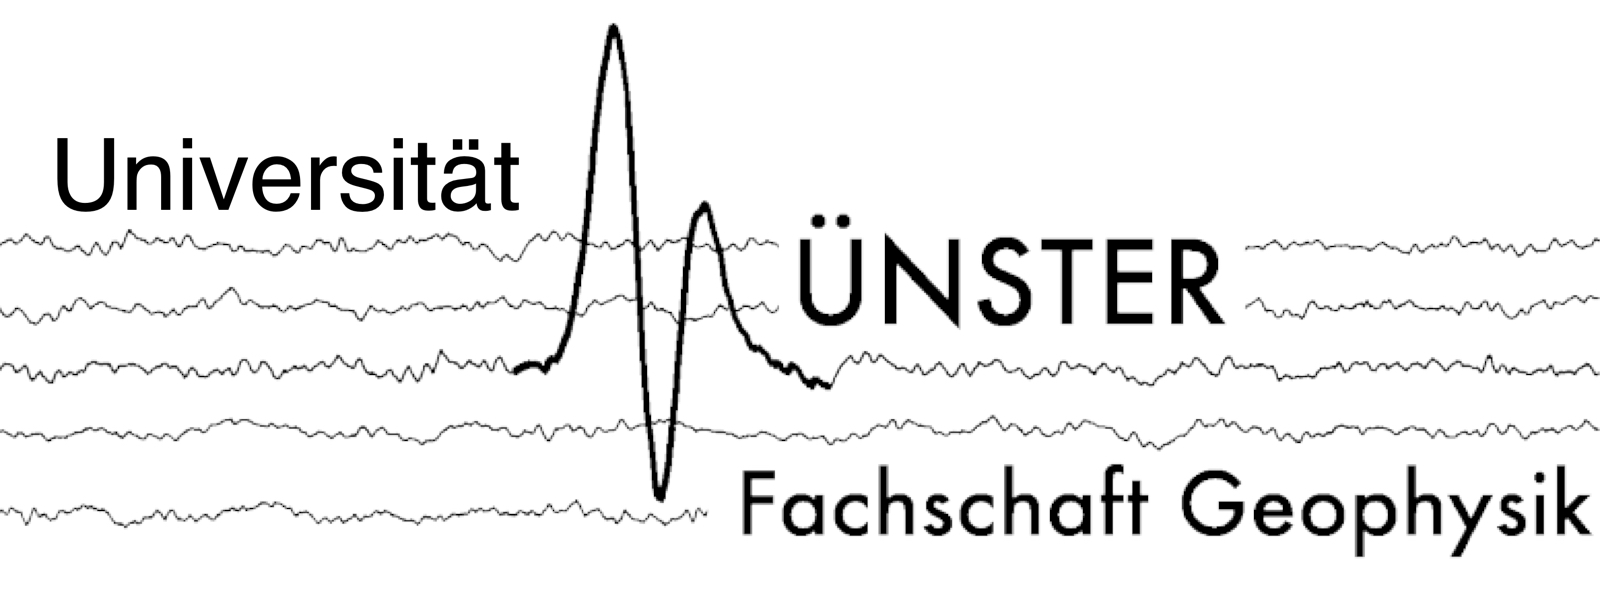
\includegraphics[width=0.8\columnwidth]{res/fs_geophysik_logo_neu.jpg}
\end{center}

Im Laufe des Jahres organisieren wir viele Veranstaltungen für Mitarbeitende und Studierende der Geophysik.
Dazu gehören insbesondere das Sommerfest, die Weihnachtsfeier, gelegentliche Exkursionen zu Institutionen und Firmen, die sich mit Geophysik beschäftigen, Vorträge von Geophysikern aus dem Berufsleben und noch einiges mehr.
Ihr seid natürlich alle herzlich eingeladen.
Eine feste Institution ist auch der monatliche Geophysik-Stammtisch:
Dazu laden wir ungefähr einmal im Monat (während der Vorlesungszeit) zu einer geselligen Runde in eine der vielen Münsteraner Kneipen ein, um über das Studium und alles Andere zu quatschen.
Auch hier könnt ihr natürlich gerne vorbeischauen und eure Kommilitonen aus den höheren Semestern kennenlernen.
Ort und Termin der Stammtische findet ihr auf unserer Internetseite:\\
\url{http://www.uni-muenster.de/Physik.GP/fachschaft/fachschaft.html}\\
Dort findet ihr natürlich auch immer alle anderen Termine und Infos rund um die Fachschaft und das Studium!

Nun zur Frage, wer wir überhaupt sind.
Ganz einfach gesprochen:
Ein bunt zusammengewürfelter Haufen von Studierenden der Geophysik, sowohl aus Bachelor- als auch Master-Studiengang; aber das ändert sich auch ständig.
Eine aktuelle Liste aller Mitglieder mitsamt Kontaktdaten findet ihr auf der Fachschaftshomepage.
Wenn ihr uns persönlich kennenlernen wollt, könnt ihr ja einmal in unserem neuen Fachschaftsraum vorbeischauen (Raum~319 im Geophysik-Institut).
Oder ihr kommt mal zu einer unserer Fachschaftssitzungen.
Diese sind nämlich öffentlich und wir freuen uns immer, wenn wir Besuch dabei haben.
Der Sitzungstermin wird immer am Anfang des Semesters festgelegt und kann auf der Homepage eingesehen werden.
Um jetzt noch ein Bild von uns zu bekommen, schaut euch einfach das Foto an.

Und wenn ihr jetzt Lust bekommen habt, auch bei der Fachschaft mitzumachen, könnt ihr ganz einfach mal zur Fachschaftssitzung kommen, uns ansprechen oder eine E-Mail schreiben (an \email{geophyf@earth.uni-muenster.de})!
Wir freuen uns immer über Verstärkung.

Auf bald, eure Fachschaft~Geophysik

\begin{subfigure}{0.4\textwidth}
    
\includegraphics[width=\textwidth]{FS_Geophysik_QR_Website2025.png}
    \caption{QR-Code zur Website.}
    \label{fig:first}
\end{subfigure}
\hfill
\begin{subfigure}{0.4\textwidth}
    
\includegraphics[width=\textwidth]{FS_Geophysik_QR_Insta2025.png}
    \caption{QR-Code zur Istagram-Seite.}
    \label{fig:second}
\end{subfigure}


%\begin{center}
%	
\includegraphics[width=0.5\columnwidth]{res/FS_Geophysik_QR_Website2025.png}
%\end{center}
\end{multicols*}

